\documentclass{beamer}
\usepackage[utf8]{inputenc}
\usepackage{url}
\usepackage{hyperref}
\graphicspath{{./fig/aula7}}

% Configurando layout para mostrar codigos C++
\usepackage{listings}
\lstset{
  language=HTML,
  basicstyle=\ttfamily\small, 
  keywordstyle=\color{blue}, 
  stringstyle=\color{red}, 
  commentstyle=\color{red}, 
  extendedchars=true, 
  showspaces=false, 
  showstringspaces=false, 
  numbers=left,
  numberstyle=\tiny,
  breaklines=true, 
  backgroundcolor=\color{green!10},
  breakautoindent=true, 
  captionpos=b,
  xleftmargin=0pt,
}


\title{Desenvolvimento Web Básico}
\subtitle{Aula 11 - Consumindo uma API}

\usetheme{lucid}

\begin{document}
\frame{
 \titlepage
}

%--------------------------------------------------------------------------
\begin{frame}{Na aula de hoje...} 
\tableofcontents 
\end{frame}
%--------------------------------------
\section{Introdução}
\begin{frame}{Formulários}
  \begin{enumerate}
      \item Formulários são utilizados na maior parte das aplicações Web para coletar dados dos usuários e registrar alterações nos mesmos;
      \item Vamos ver como sincronizar um formulário para consumir uma API pública;
  \end{enumerate}
\end{frame}
%--------------------------------------
\section{Formulário}
\begin{frame}{Formulários}
Construa um formulário como o apresentado abaixo:
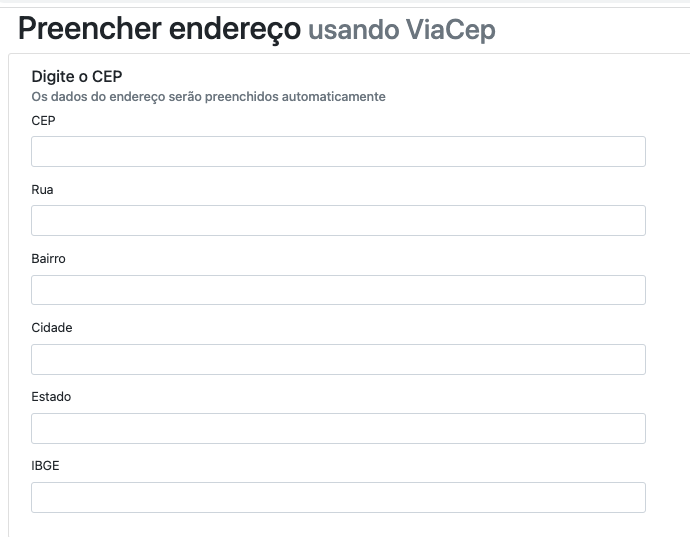
\includegraphics[height=0.6\paperheight]{fig/aula11/aula11_1.png}
Código disponível na aula 12 (Github - branch 2023).
\end{frame}
%--------------------------------------
\section{Javascript}
\begin{frame}{Ações}
Note que temos a tag form, e nela a ação definida é GET.
\\
\begin{itemize}
    \item Ao digitar o CEP nossa input tem uma ação definida \textbf{onblur}. Que chama a função \textit{pesquisacep()} e passa o valor do campo por parâmetro.
\end{itemize}
\end{frame}
%--------------------------------------
\begin{frame}{pesquisacep}
A API ViaCep funciona da seuinte forma.
\\
\begin{itemize}
    \item A rota de GET para a URL: \url{https://viacep.com.br/ws/} espera como parâmetro um valor de CEP e o formato que desejamos receber a resposta;
    \item Digamos que você queira consultar o CEP \textbf{86020-080};
    \item A URL de GET será \url{https://viacep.com.br/ws/86020080/json/}
    \item A resposta será em formato JSON. 
    \item No nosso formulário, vamos substituir o 86020080 por uma variável que vai conter o valor digitado pelo usuário;
\end{itemize}
\end{frame}
%-----------------------------------------------------------------
\section{Atividade de aula}
\begin{frame}{Atividade}{Envie seu repositório feito em aula}
  \begin{enumerate}
      \item Seguindo os passos da aula, livros indicados e, a leituras recomendadas:
      \item Desenvolva um formulário de sua preferência que contenha os campos exibidos e monte um texto com as seleções do usuário.
      \item Além disso o formulário deve mudar as cores com base em combinações de seleção diferentes;
      \item Aplique CSS com Bootstrap para posicionamento e tipografia de elementos conforme a aula anterior
  \end{enumerate}


\end{frame}
%-----------------------------------------------------------------------
\section{Leitura recomendada}
\begin{frame}{Leitura complementar}
 Para mais informações sobre Git e GitHub, leia:\\
  \vspace{0.6cm}
 \begin{columns}
   \begin{column}{0.4\textwidth}
%      \textbf{Capítulo 29}\\
 \cite{githubpages2022}\\
 E\\
 \cite{beer2015github}.
   \end{column}
   \begin{column}{0.4\textwidth}
   % 
\includegraphics[height=0.7\paperheight]{introgit.jpg} \\
   \end{column}

 \end{columns}
\end{frame}

%----------------------------------------------------------------------------
\section{Referências}

\begin{frame}{Referências}%[allowframebreaks]
\small
\begin{center}
\tiny
\bibliographystyle{apalike}
\bibliography{ref_aula}
\end{center}
\end{frame}

\end{document}